% Compile from this directory with: xelatex why_three_stage1.tex
\documentclass[11pt,a4paper]{article}
\usepackage{kotex}
\usepackage{amsmath,amssymb,booktabs,graphicx,geometry,hyperref}
\geometry{margin=25mm}
\graphicspath{{../results/}}
\hypersetup{colorlinks=true,urlcolor=blue,linkcolor=blue}

\title{I01 후속 실험 1: 왜 3인가?\\국소 조우의 임계차원과 선택 창}
\author{문헌 대조 및 재현 가능한 계산 실험}
\date{2026년 10월 2일}

\begin{document}
\maketitle

\begin{abstract}
``왜 공간방향이 3개인가''는 문헌에 제안이 없어서 생긴 질문이 아니다.
서로 다른 모형이 조건부로 3을 산출하지만, 초기조건과 동역학 가정이
검증되지 않았거나 근사/변형에 민감하다. 본 노트는 I01의 대각 제약과
다른 계열인 끈 감김 소멸 기작에서, 3이 나오는 \emph{기하학적 필요조건}
을 독립적인 국소 조우 토이로 확인한다. 조건부 Poisson 단계 모형은
3에서 멈출 수 있는 창을 정량화한다. 어느 결과도 감김 소멸, 우주 팽창,
실재 공간차원 발생의 증거로 해석하지 않는다.
\end{abstract}

\section{문헌에서 이미 알려진 것과 남은 간극}
Brandenberger--Vafa 계열의 핵심은 감긴 끈과 반감긴 끈이 만나
소멸해야 공간방향이 크게 자랄 수 있다는 가설이다.
9-토러스의 특정 초기조건을 연구한 Easther 등은 3개의 큰 방향이
가능하지만 통계적으로 선호되지는 않는다고 보고했다 \cite{Easther2005}.
반면 Greene 등은 연속 열적 요동과 충분한 끈 결합 세기라는
조건에서 3개 방향이 선호됨을 보였고, 요동의 동역학/통계에
추가 연구가 필요하다고 명시했다 \cite{Greene2013}.
따라서 ``문헌이 3을 확정하지 못했다''는 진술은 타당하지만,
``3을 선택하는 기존 기작이 없다''는 진술은 틀리다.

별도 계열인 Lorentzian type-IIB 행렬모형에서는 3+1차원 팽창상이
수치적으로 보고되었다. 이전 근사에서 얻은 팽창공간의 일부 구조가
근사 인공물일 수 있다는 분석도 있다 \cite{Aoki2019}.
2026년의 복소 Langevin 계산은 \emph{변형된} 모형의 매끄러운
3+1차원 팽창상을 보고한다 \cite{Matrix2026}. 이것은 흥미로운
경쟁 가설이지, 원래의 I01 대각 제약이나 실제 우주에 대한 확증은 아니다.

\section{사전등록한 국소 조우 토이}
$d$개의 국소 공간좌표에서 두 개의 움직이는 1차원 끈 조각을
\begin{align}
x_A(t,s_A)&=c_A+v_A t+u_A s_A,\\
x_B(t,s_B)&=c_B+v_B t+u_B s_B
\end{align}
로 놓는다. 같은 시간에 만나려면
\begin{equation}
A z=b,\qquad
A=(v_A-v_B,\;u_A,\;-u_B)\in\mathbb R^{d\times3},\quad
z=(t,s_A,s_B)^T,\quad b=c_B-c_A
\end{equation}
를 만족해야 한다. 세 매개변수의 허용범위는 모두
$[-1/2,1/2]$로 제한한다. $A$의 성분은 독립 $N(0,1)$,
$b$의 성분은 독립 $N(0,\sigma^2)$로 뽑는다.
접촉 두께 $\delta$에서의 사건은 최소제곱 해 $\hat z$가
허용 상자 안에 있고 $\|A\hat z-b\|<\delta$인 것이다.
이는 \emph{내부 최단접근} 사건만 세므로 경계 접촉을 모두
포함한 실제 끈 충돌확률은 아니다. 또한 감김, 토러스 주기영상,
상호작용과 우주 팽창을 포함하지 않는다.

$d=3$에서는 거의 모든 $A$가 역행렬을 가져 내부해가 존재하는
비영 확률 $q_3$가 남는다. $d>3$에서는 나머지 $d-3$개
직교 방향의 거리가 접촉 두께보다 작아야 한다. 등방 Gaussian
오프셋에서는 투영 성분과 직교 성분이 독립이므로 정확히
\begin{equation}
p_d(\delta)=q_d F_{\chi_{d-3}}(\delta/\sigma),\quad
q_d=\Pr(\hat z\in[-1/2,1/2]^3),\qquad d\ge3,
\end{equation}
여기서 $F_{\chi_0}=1$로 정의한다. 따라서
\begin{equation}
p_d(\delta)\propto\delta^{d-3}\quad(d>3,\;\delta\ll\sigma).
\end{equation}
이 지수는 세계면 조우의 차원 계산을 재확인한 것이며,
새로운 우주론 예측이 아니다.

\section{재현 실험의 결과}
주 계산은 $\sigma=0.35$, 차원당 150,000개 독립 표본,
고정 seed 20261002를 썼다. $\delta=0.005,0.01,0.02$에서
$\log p$--$\log\delta$ 기울기를 적합했다.
\begin{center}
\begin{tabular}{@{}ccccc@{}}
\toprule
공간방향 $d$ & 3 & 4 & 5 & 6\\
\midrule
예측 지수 $d-3$ & 0 & 1 & 2 & 3\\
측정/해석적 조합 기울기 & 0.000 & 0.9996 & 1.9994 & 2.9993\\
내부해 확률 $q_d$ & 0.3908 & 0.6494 & 0.7994 & 0.8873\\
\bottomrule
\end{tabular}
\end{center}
기울기는 $q_d$를 Monte Carlo로 구하고 직교 잔차의 정확한
$\chi$ 분포를 곱한 Rao--Blackwell 추정량에서 나온다.
별도의 직접 충돌 계수도 이 값과 일치하는지 검사했다.
$\sigma=0.25,0.5$의 대조 계산에서도 작은 두께의 지수는 유지된다.
단, 확률의 절대 크기는 $\sigma$, 조각 길이, 속도 분포에 달려 있다.

\section{필수 대조군: 두 접선이 평행하면 3의 경계가 달라진다}
위 결과는 두 끈의 국소 접선이 독립이라는 조건을 사용했다.
정확히 곧고 평행한 두 감김 끈을 가정하면 $u_B=u_A$이고,
$(s_A,s_B)$는 상대좌표 하나로 합쳐진다. 만남의 독립 매개변수는
$(t,s_A-s_B)$ 두 개가 되므로 직교 여차원은 $d-2$이다.
따라서 두께 $\delta\to0$에서
\begin{equation}
p_d^{\rm aligned}(\delta)\propto\delta^{d-2}.
\end{equation}
특히 정확히 평행한 경우의 $d=3$ 조우 확률은 유한한 상수가
아니라 $\delta$에 비례해서 0으로 간다. 감김 방향이 같다고 해서
현실의 끈 접선이 반드시 평행한 것은 아니다. 진동과 굴곡이
있다면 접선이 독립될 수 있지만, 그 분포는 동역학에서 유도해야 한다.

이를 검사하기 위해 $u_B=u_A+\eta\xi$를 넣고 $\eta=0,0.01,0.1,1$
을 비교했다. 두/세 매개변수 상자에서 \emph{경계면까지 포함한}
최소거리를 정확한 active-set 열거로 구했다.
$d=3$에서 $\eta=0$의 유한두께 로그기울기는
$\delta=0.005$--0.02 범위에서 약 0.99였다.
$\eta=0.01,0.1,1$에서는 각각 약 $0.79,0.28,0.06$이었다.
반면 $\eta>0$을 고정하고 $\delta\to0$을 먼저 취하면
기울기는 0이고, 내부에서의 영두께 조우확률은
$\eta=0.01,0.1,1$에서 각각 약 $0.0053,0.0499,0.316$이다.
즉 약한 요동에서는 유한두께 crossover가 길게 남으며,
$\eta\to0$과 $\delta\to0$ 극한의 순서를 구분해야 한다.
표본 집합, patch 크기와 접선 요동 법칙에 수치가 의존한다.

\begin{figure}[ht]
\centering
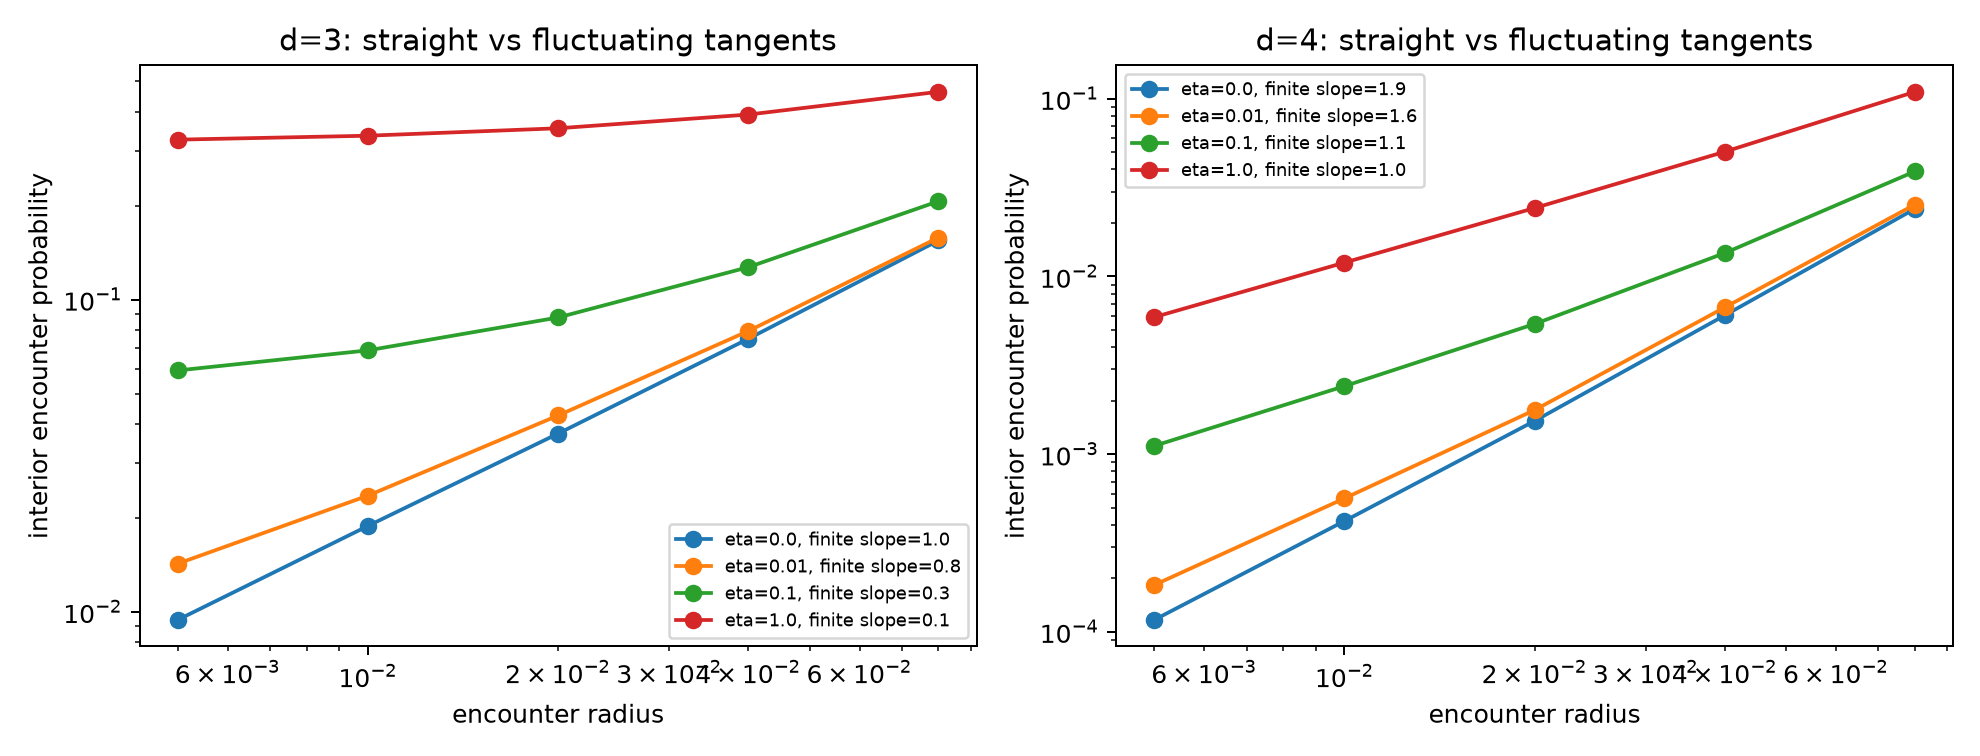
\includegraphics[width=\textwidth]{tangent_alignment.png}
\caption{정확히 평행한 접선과 횡방향 요동 접선의 비교.
표시한 기울기는 유한 두께 범위의 Monte Carlo 적합이며
엄밀한 $\delta\to0$ 지수와 다를 수 있다.}
\end{figure}

\section{3에서 멈추는 창은 추가 동역학 가정을 필요로 한다}
국소 접촉이 실제 감김 소멸을 일으켜 다음 차원이 자랄 수 있다고
\emph{추가로 가정}하자. 또한 3차원 단계에 이미 도달했고,
3차원과 4차원 단계 각각에서 평균 $M$회의 독립적인 접촉 기회가
Poisson 분포를 따른다고 놓는다. 이때
\begin{equation}
P_{\rm stop\,3}(M)=(1-e^{-Mp_3})e^{-Mp_4}.
\end{equation}
$\delta=0.005$에서는 $p_3=0.3908$, $p_4=0.00740$이며,
비율은 52.8이다. $M\simeq10.2$에서 조건부 정지 확률의 최댓값은
0.910이다. 두께가 0.02이면 같은 최댓값은 0.760,
0.08에서는 0.495로 떨어진다. 특히 3단계 성공확률 90\% 이상과
4단계 성공확률 10\% 이하를 동시에 원하면
\begin{equation}
\frac{p_3}{p_4}\ge\frac{-\ln(0.1)}{-\ln(0.9)}\simeq21.85
\end{equation}
가 필요하다. 이 표본 설정에서는 두께 0.005와 0.01은 이 조건을
만족하지만 0.02는 만족하지 않는다.

이 숫자들은 \emph{3단계 도달을 조건으로 한} 가짜 단계모형의
성공확률이다. 실제 초기 차원 분포, 감김 수밀도, 팽창시간,
끈 결합, 산란/재결합 확률을 넣지 않았으므로 우주가 3차원으로
끝날 확률이 아니다. 얇은 끈에서 4차원 접촉이 억제된다는
필요조건은 확인되지만, 충분조건은 확인되지 않았다.

\begin{figure}[ht]
\centering
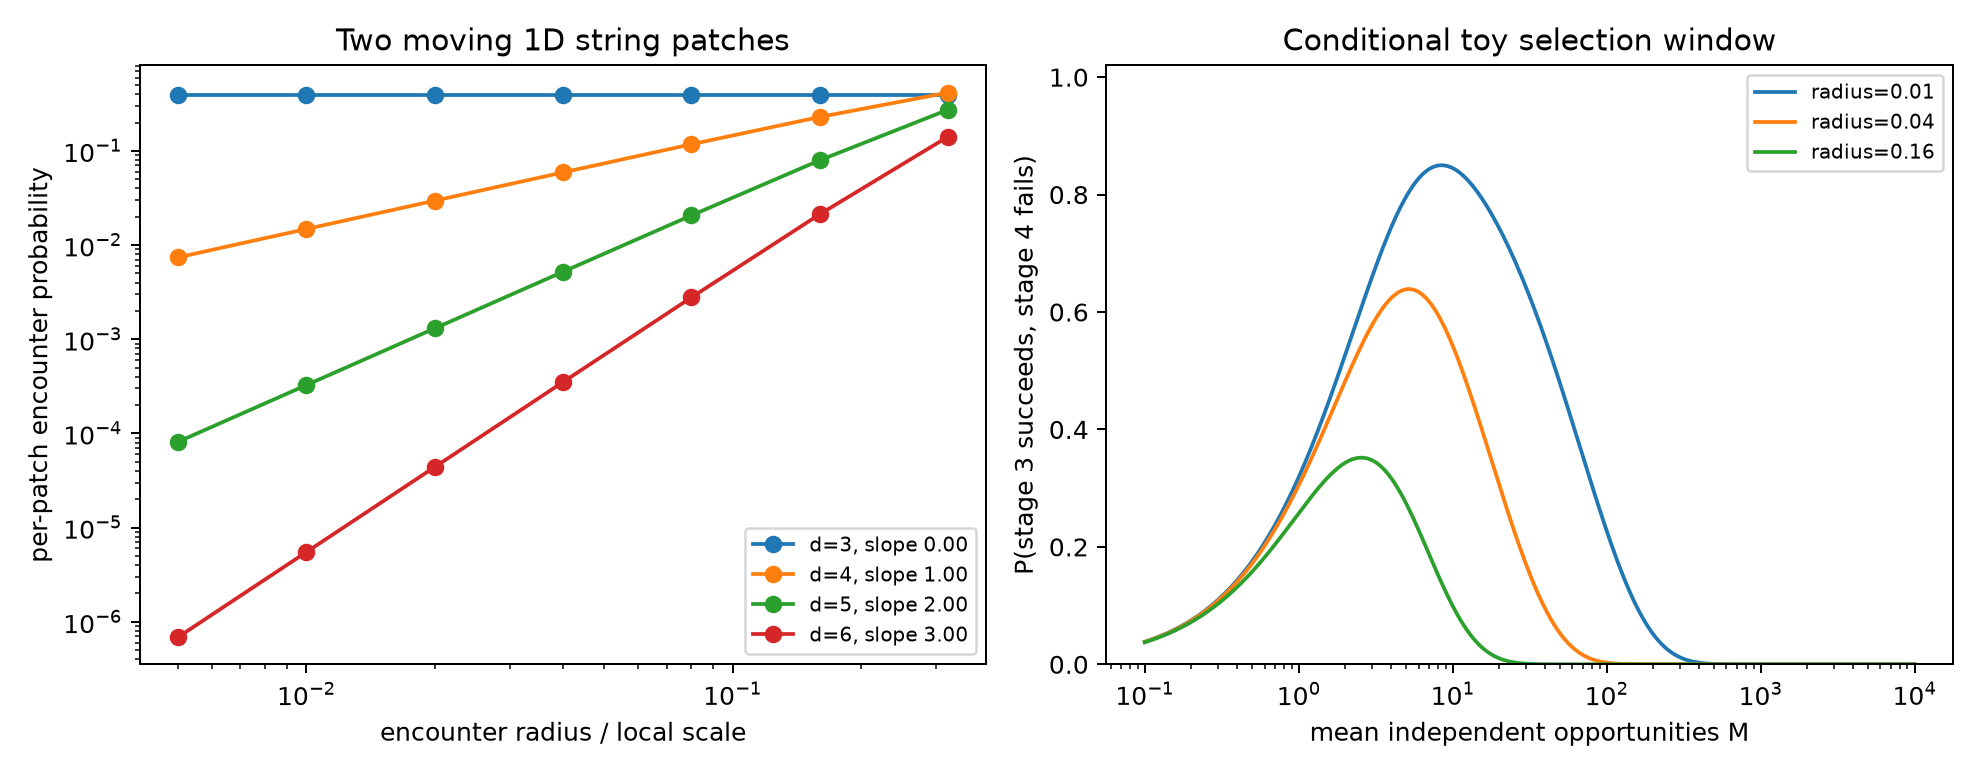
\includegraphics[width=\textwidth]{encounter_threshold.png}
\caption{왼쪽: 국소 조우 확률의 두께 의존성. 오른쪽: 별도
Poisson 단계 가정 아래의 조건부 3단계 정지 창.}
\end{figure}

\section{I01에 대한 결정과 다음 실험}
I01의 단일 대각 $U(1)$ 제약은 $n-1$방향을 남겨 3을 일반적으로
고르지 못한다. 반면 움직이는 1차원 객체의 조우 기하에는
$d=3$ 경계가 \emph{동역학을 추가하기 전부터} 있다.
이 둘을 같은 효과로 부르지 말고, 후자를 I01의 ``왜 3''에 대한
경쟁 기준선으로 둔다. I01이 새로운 설명이 되려면 단순 rank 3이
아니라 기존 조우 기작과 다른 구별 예측을 내야 한다.

다음 단계는 보존되는 감김 수를 가진 객체를 실제 $T^n$ 위에서
움직이게 하여 접촉--소멸과 반지름 팽창을 결합하는 것이다.
차원별 초기조건을 동일하게 샘플링하고, 접촉 두께, 수밀도,
팽창속도, 관측기간을 바꾼다. 그 뒤 각 시점의 물질 전파/
스펙트럼 차원과 I01의 조건부 Fisher 차원을 \emph{같은 실현}
에서 비교해야 한다. 3이 넓은 모수 영역에서 살아남지 않거나
검출기 변화로만 생기면 ``왜 3''의 후보 메커니즘으로 기각한다.

\paragraph{재현성.} 계산 코드는 \texttt{../src/relational\_atlas\_i01/geometry/encounter\_threshold.py},
결과 JSON은 \texttt{../results/encounter\_threshold.json}이다.
코드와 직접 Monte Carlo/투영항등식 일치 여부의 테스트는
\texttt{../tests/test\_encounter\_threshold.py}에 있다.
접선 평행성 대조군은 \texttt{../src/relational\_atlas\_i01/geometry/tangent\_alignment.py},
그 결과는 \texttt{../results/tangent\_alignment.json},
테스트는 \texttt{../tests/test\_tangent\_alignment.py}에 있다.

\begin{thebibliography}{9}
\bibitem{Easther2005} R. Easther, B. R. Greene, M. G. Jackson,
and D. Kabat, ``String windings in the early universe,''
\emph{JCAP} \textbf{0502}, 009 (2005),
\url{https://arxiv.org/abs/hep-th/0409121}.
\bibitem{Greene2013} B. Greene, D. Kabat, and S. Marnerides,
``On three dimensions as the preferred dimensionality of space via
the Brandenberger--Vafa mechanism,'' \emph{Phys. Rev. D} \textbf{88},
043527 (2013), \url{https://arxiv.org/abs/1212.2115}.
\bibitem{Aoki2019} T. Aoki et al., ``On the structure of the emergent
3d expanding space in the Lorentzian type IIB matrix model,''
\emph{Prog. Theor. Exp. Phys.} (2019),
\url{https://arxiv.org/abs/1904.05914}.
\bibitem{Matrix2026} K. N. Anagnostopoulos et al.,
``The emergence of (3+1)-dimensional expanding spacetime from complex
Langevin simulations of the Lorentzian type IIB matrix model with
deformations,'' arXiv:2604.19836 (2026),
\url{https://arxiv.org/abs/2604.19836}.
\end{thebibliography}
\end{document}
